% Source: phaseTransitions_liquidCrystals.pdf, pages 1-7. Title on the source: "Other types of phase
% transitions". The notes carry no lecture number.
So far, we have discussed phase transitions and critical phenomena in a number of different systems, including
liquid--gas, solid--liquid, magnetic (FM or AFM) materials, superconductors, and superfluids. We proceed to discuss
additional types of phase transitions.

\subsection{Liquid crystals}

Of considerable interest, both theoretically and in applications, are liquid crystals. These exhibit properties
that are intermediate between solids and liquids. They are of several types: nematic, smectic, cholesteric, and
discotic. The first three are composed of rod-like molecules which are long and rather rigid. A simple model
depicts these as rods. In the disordered phase, these rod-like molecules are free to move around in the liquid (often
in a solvent) subject to excluded-volume constraints, and are oriented randomly. This phase is called the isotropic
phase. As a function of temperature $T$ for thermotropic liquid crystals, or concentration $c$ for lyotropic liquid
crystals (LCs), as $T$ decreases below $T_{p.t.}$ or $c$ increases past $c_{p.t.}$, there is a phase transition from the
isotropic to the nematic phase.

\begin{diagram}
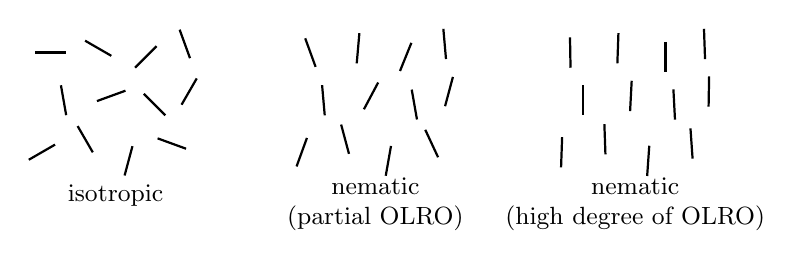
\begin{tikzpicture}[scale=0.55]
  \foreach \x/\y/\a in {0/0/30,1/0.3/120,2/-0.2/75,3/0.2/160,0.5/1.2/100,1.6/1.3/20,2.6/1.1/135,3.4/1.4/60,0.2/2.3/0,1.3/2.4/150,2.4/2.2/45,3.3/2.5/110}
    \draw[thick] (\x,\y) ++(\a:0.35) -- ++(\a+180:0.7);
  \node[font=\small] at (1.7,-1) {isotropic};
  \begin{scope}[xshift=6cm]
  \foreach \x/\y/\a in {0/0/70,1/0.3/105,2/-0.2/80,3/0.2/115,0.5/1.2/95,1.6/1.3/62,2.6/1.1/100,3.4/1.4/75,0.2/2.3/110,1.3/2.4/85,2.4/2.2/68,3.3/2.5/95}
    \draw[thick] (\x,\y) ++(\a:0.35) -- ++(\a+180:0.7);
  \node[font=\small,align=center] at (1.7,-1.2) {nematic\\ (partial OLRO)};
  \end{scope}
  \begin{scope}[xshift=12cm]
  \foreach \x/\y/\a in {0/0/88,1/0.3/92,2/-0.2/86,3/0.2/94,0.5/1.2/90,1.6/1.3/87,2.6/1.1/93,3.4/1.4/89,0.2/2.3/91,1.3/2.4/88,2.4/2.2/90,3.3/2.5/92}
    \draw[thick] (\x,\y) ++(\a:0.35) -- ++(\a+180:0.7);
  \node[font=\small,align=center] at (1.7,-1.2) {nematic\\ (high degree of OLRO)};
  \end{scope}
\end{tikzpicture}
\diagramcaption{2D slices through the actual 3D liquids in the isotropic and nematic phases. OLRO = orientational
long-range order.}
\end{diagram}

In the nematic phase, the LC exhibits orientational long-range order, but, as in the isotropic phase, no positional
ordering within the liquid. In the simplified description in terms of rods, the space of the order parameter for this
isotropic-to-nematic phase transition is
\begin{equation}
  P^2 = S^2/\mathbb{Z}_2,
\end{equation}
where $S^2$ is the 2-sphere and we mod out by $\mathbb{Z}_2$ because the ends of the rods are equivalent.
$P^N = S^N/\mathbb{Z}_2$ is the $N$-dimensional projective space. This $P^2$ topological space may be contrasted with the
$S^2$ space of the order parameter $\mathbf M = \ev{\mathbf S}$ of the FM $O(3)$ spin model in $d = 3$, with magnetization
$\mathbf M = \ev{(S_x,S_y,S_z)}$ (rods vs.\ arrows).

A physical mechanism for this phase transition (discussed by Onsager) is that with the rods lined up, at least
partially, there is less obstruction in their motion; they undergo fewer collisions, especially for motion in the
$\hat{\mathbf n}$ direction, where $\hat{\mathbf n}$ is the axis (equivalent under $\hat{\mathbf n}\to-\hat{\mathbf n}$)
along which the nematic ordering takes place. In contrast, in the isotropic phase rods have a higher tendency to collide
with each other as they move.

\subsubsection*{Model Hamiltonian and order parameter}

A model Hamiltonian for a nematic LC has a rod--rod interaction energy favoring alignment of nearest-neighbor rods. To
take into account the $\hat{\mathbf n}\leftrightarrow-\hat{\mathbf n}$ equivalence, one can use regular 3D vectors
$\hat{\mathbf S}_i$ but square the scalar product, so
\begin{equation}
  E_{ij} = -J(\hat{\mathbf S}_i\cdot\hat{\mathbf S}_j)^2 = -J\cos^2(\theta_i-\theta_j),
\end{equation}
where $\theta_i-\theta_j$ is the angle between $\hat{\mathbf S}_i$ and $\hat{\mathbf S}_j$ (with $|\hat{\mathbf S}_i| = 1$:
unit normalization).

An order parameter, defined to be zero in the isotropic phase and nonzero in the nematic phase, is the scalar order
parameter
\begin{equation}
  s = \frac{1}{2}(3\cos^2\theta-1),
\end{equation}
where here, $\theta$ is the polar angle of the rods with respect to the ordering axis $\hat{\mathbf n}_0\sim\hat{\mathbf z}$.
For example, if this axis is taken to be the $\hat{\mathbf z}$ axis, then with the usual spherical coordinates one has
$\int\dd\Omega = \int_0^\pi\sin\theta\,\dd\theta\int_0^{2\pi}\dd\phi = 2\pi\int_{-1}^1\dd\cos\theta = 2\pi\int_{-1}^1\dd\xi$.
Note that $s = P_2(\cos\theta)$, where $P_\ell(\cos\theta)$, with $\xi = \cos\theta$, is the $\ell$'th Legendre polynomial.
Recall: $P_0(\xi) = 1$, $P_1(\xi) = \xi$, $P_2(\xi) = (1/2)(3\xi^2-1)$, $P_3(\xi) = (1/2)(5\xi^3-3\xi)$, etc.,
\begin{equation}
  P_\ell(\xi) = \frac{1}{2^\ell\ell!}\frac{\dd^\ell}{\dd\xi^\ell}(\xi^2-1)^\ell;\qquad P_\ell(1) = 1,
\end{equation}
and the inner product in the function space is
\begin{equation}
  \langle P_\ell,P_{\ell'}\rangle = \int_{-1}^1\dd\xi\,P_\ell(\xi)P_{\ell'}(\xi) = \frac{2}{2\ell+1}\delta_{\ell\ell'} .
\end{equation}
Thus in the isotropic phase,
$\ev s = \int_{-1}^1\dd\xi\,s(\xi) = \int_{-1}^1\dd\xi\,P_2(\xi)\cdot\underbrace{P_0(\xi)}_{1} = 0$. In the limit of
complete orientational ordering, $\cos\theta = 1$, $s = 1$. The full range of values of $s$ extends from $s = -1/2$
for $\theta = \pi/2$ to $s = 1$ for $\theta = 0$.

The partition function is then (for a thermotropic LC)
\begin{equation}
  Z\sim\int\left[\prod_i\frac{\dd\Omega_i}{(4\pi)}\right]e^{-\beta\Ham},\qquad
  \Ham = -J\sum_{ij}P_2\left(\cos(\theta_i-\theta_j)\right).
\end{equation}

\subsubsection*{Order of the isotropic--nematic transition}

The order of the isotropic-to-nematic phase transition can be seen from the Landau--Ginzburg free energy function:
\begin{equation}
  A = L_0 + L_1s + L_2s^2 + L_3s^3 + L_4s^4 .
\end{equation}
The constant term $L_0$ does not affect the determination of the minimum of $A$ as a function of $s$. The coefficient of
the linear term $L_1 = 0$, since otherwise $\left.\partial A/\partial s\right|_{s=0}\ne 0$ and $s = 0$ would not minimize
$A$ even in the isotropic phase. So
\begin{equation}
  A = L_2s^2 + L_3s^3 + L_4s^4,
\end{equation}
where $L_i = L_i(T)$ for a thermotropic LC and $L_i = L_i(c)$ for a lyotropic LC. The cubic term is present because the
physics is not invariant, even in the isotropic phase, under $s\to-s$. This is in contrast to the $O(3)$ spin model, where
$Z$ is invariant under $\mathbf M\to-\mathbf M$ (indeed it is invariant under a rotation $\mathbf M\to R\mathbf M = \mathbf M'$).
The presence of the cubic term leads to a first-order phase transition. This is confirmed in Monte Carlo simulations.
These naturally freeze out the orientational degrees of freedom and hence assign sites to the centers of the rods, so
\begin{equation}
  \Ham = -J\sum_{e_{ij}}\frac{1}{2}\left[3(\hat{\mathbf S}_i\cdot\hat{\mathbf S}_j)^2-1\right] = -J\sum_{e_{ij}}P_2\left(\cos(\theta_i-\theta_j)\right).
\end{equation}

\begin{diagram}
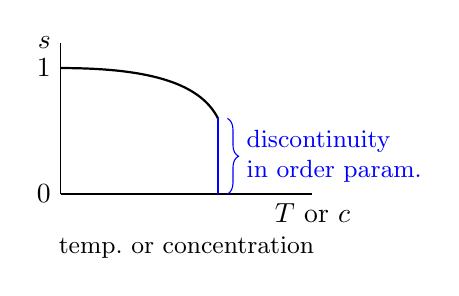
\begin{tikzpicture}[scale=0.8]
  \draw (0,0) -- (4,0) node[below] {$T$ or $c$}; \draw (0,0) -- (0,2.4) node[left] {$s$};
  \draw[thick] (0,2) .. controls (1.3,2) and (2.2,1.8) .. (2.5,1.2);
  \draw[thick,blue] (2.5,1.2) -- (2.5,0);
  \node[left] at (0,2) {$1$}; \node[left] at (0,0) {$0$};
  \draw[blue,decorate,decoration={brace,amplitude=4pt}] (2.65,1.2) -- (2.65,0);
  \node[blue,anchor=west,font=\small,align=left] at (2.8,0.6) {discontinuity\\ in order param.};
  \node[below=12pt,font=\small] at (2,0) {temp.\ or concentration};
\end{tikzpicture}
\diagramcaption{First-order isotropic--nematic transition.}
\end{diagram}

Just as the $O(3)$ spin model can be abstractly generalized to an $O(N)$ spin model, so also one may study an abstract
$P^N$ nematic liquid crystal model; see G.~Kohring and R.~Shrock, Nucl.\ Phys.\ B \textbf{285}, 504 (1987). As with the
$P^2$ case, the $P^N$ LC also exhibits a 1st-order phase transition. See also G.~Kohring and R.~Shrock, Nucl.\ Phys.\ B
\textbf{295}, 36 (1988) for further study.

\subsubsection*{Real liquid-crystal molecules and displays}

In actual nematic LCs, although the simplifying approximation of representing the molecule as a rigid rod is reasonably
good at describing several physical properties, the molecules are not precisely invariant under inversion. We show some
examples: e.g.\ biphenyl nitriles,
\begin{equation*}
  \mathrm{C_7H_{15}}\!-\!\left\langle\bigcirc\right\rangle\!-\!\left\langle\bigcirc\right\rangle\!-\!\mathrm{C{\equiv}N},
  \qquad
  \mathrm{C_8H_{17}}\!-\!\mathrm{O}\!-\!\left\langle\bigcirc\right\rangle\!-\!\left\langle\bigcirc\right\rangle\!-\!\mathrm{C{\equiv}N},
\end{equation*}
where $\langle\bigcirc\rangle$ denotes a benzene ring (a linear combination of the two Kekul\'e structures of
C$_6$H$_4$, with alternating single and double bonds) and C$_7$H$_{15}$ is the heptyl chain
H$-$(CH$_2$)$_6-$CH$_2-$, drawn as a zigzag in standard chemical notation.

The CN endgroup is polar, so these LC molecules can be oriented by an applied electric field. In a typical application to
a black and white (actually black and grayish-white) numerical display in a digital watch or hand calculator, light is
passed through a polarizing filter, followed by a layer of nematic LCs subject to electric fields. In a twisted nematic
LC (TNLC) cell between horizontal and vertical polarizing filters, the twisted LC rotates the polarization, so the light
passes through and the screen is bright gray. When the field is applied, light is polarized by the horizontal polarizing
filter and since the LCs are longitudinally oriented, they do not change the polarization, so the light is blocked by the
vertical polarization filter, producing a dark screen. The cells have a pixelated structure.

\begin{diagram}
\begin{tikzpicture}[scale=0.6,>=Stealth]
  \foreach \s/\on in {0/0,8/1} {
  \begin{scope}[xshift=\s cm]
    \draw (0,0) -- (5,0) -- (6,1) -- (6,3) -- (1,3) -- (0,2) -- cycle; \draw (0,2) -- (5,2) -- (6,3); \draw (5,0) -- (5,2);
    \foreach \y in {0.6,1.0,1.4} \draw (0.15,\y) -- (0.85,\y+0.2);
    \foreach \x in {5.25,5.5,5.75} \draw (\x,0.6) -- (\x,1.9);
    \ifnum\on=0
      \foreach \x/\a in {1.6/10,2.3/35,3.0/60,3.7/85} \draw[blue,thick] (\x,1.4) ++(\a:0.35) -- ++(\a+180:0.7);
      \node[blue,font=\scriptsize,align=center] at (3,3.6) {light passes through,\\ screen is bright gray};
    \else
      \foreach \x in {1.6,2.3,3.0,3.7} \draw[blue,thick] (\x-0.35,1.4) -- (\x+0.35,1.4);
      \node[blue,font=\scriptsize] at (3,3.5) {light is blocked};
    \fi
    \draw[->,red,thick] (1.2,0.6) -- (2.6,0.6);
  \end{scope}}
  \node[red,font=\scriptsize] at (1.5,-0.5) {direction of light propagation};
\end{tikzpicture}
\diagramcaption{Schematic twisted nematic LC (TNLC) display cell between horizontal and vertical polarizing filters,
without (left) and with (right) the applied field.}
\end{diagram}

LC diode (LCD) displays quickly replaced cathode ray tubes (CRTs) in the 1990s for computer monitors, since LCDs take much
less power, run cooler, and are much smaller and lighter. They are also used in laptop and iPad displays (with color LEDs
to provide color illumination).

\subsubsection*{Other types of liquid crystals}

Other types of liquid crystals, with pictures of ordered states:
\begin{itemize}
  \item \emph{Smectic LC.} In this type of LC, when the system goes from the isotropic phase to the smectic phase the LC
    rod-like molecules not only exhibit a nonzero $\ev s$, orientational LRO; they also exhibit partial positional
    ordering in layers orthogonal to the axis $\hat{\mathbf n}_0$ of rod alignment.
  \item \emph{Cholesteric LC.} In this case the $\hat{\mathbf n}_0$ in the layers shifts as a function of $\hat{\mathbf z}$.
  \item \emph{Discotic LC.} This type of LC consists of disk-like molecules.
\end{itemize}

\begin{diagram}
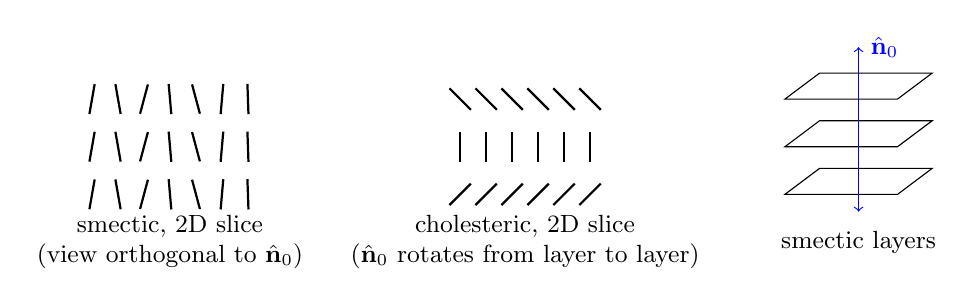
\begin{tikzpicture}[scale=0.55]
  \foreach \r in {0,1,2} \foreach \x/\a in {0/80,0.6/100,1.2/75,1.8/95,2.4/105,3.0/85,3.6/92}
    \draw[thick] (\x,1.1*\r) ++(\a:0.35) -- ++(\a+180:0.7);
  \node[font=\small,align=center] at (1.8,-1.1) {smectic, 2D slice\\ (view orthogonal to $\hat{\mathbf n}_0$)};
  \begin{scope}[xshift=8.5cm]
    \foreach \r/\a in {0/45,1/90,2/135} \foreach \x in {0,0.6,1.2,1.8,2.4,3.0}
      \draw[thick] (\x,1.1*\r) ++(\a:0.35) -- ++(\a+180:0.7);
    \node[font=\small,align=center] at (1.5,-1.1) {cholesteric, 2D slice\\ ($\hat{\mathbf n}_0$ rotates from layer to layer)};
  \end{scope}
  \begin{scope}[xshift=16cm]
    \foreach \y in {0,1,2} \draw (0,1.1*\y) -- (2.6,1.1*\y) -- (3.4,1.1*\y+0.6) -- (0.8,1.1*\y+0.6) -- cycle;
    \draw[<->,blue] (1.7,-0.4) -- (1.7,3.4); \node[blue,font=\small] at (2.3,3.4) {$\hat{\mathbf n}_0$};
    \node[font=\small] at (1.7,-1.1) {smectic layers};
  \end{scope}
\end{tikzpicture}
\diagramcaption{Ordered states of smectic and cholesteric liquid crystals.}
\end{diagram}

\subsubsection*{Comparative summary of properties of these phases of matter}

\begin{center}
\small
\renewcommand{\arraystretch}{1.25}
\begin{tabular}{>{\raggedright}p{0.17\linewidth}>{\raggedright}p{0.17\linewidth}>{\raggedright}p{0.22\linewidth}>{\raggedright}p{0.1\linewidth}>{\raggedright\arraybackslash}p{0.2\linewidth}}
  property & solid & liquid crystal & liquid & gas\\ \hline
  positional ordering & yes & no for isotropic/nematic; partial ordering in layers for smectic, cholesteric & no & no\\[2pt]
  orientational ordering & depends on substance; yes for many; no for H$_2$O ice & no in isotropic phase; yes in nematic, smectic, and cholesteric phases & no & no\\[2pt]
  is flow possible & no (although, e.g., some flow can occur in glasses over very long time scales) & yes & yes & yes\\[2pt]
  confinement of particles in volume & yes & yes & yes & no: the gas expands to fill the container\\[2pt]
  compressibility & small & small & small & large
\end{tabular}
\end{center}
N.B.: There are also other phases of matter, including (1) plasma, for $\kB T>$ few eV (where atoms and molecules are
ionized), and (2) QGP, quark--gluon plasma, for $\kB T\gtrsim 200$~MeV, where quarks and gluons are deconfined.

\subsection{Disorder, frustration and ground-state entropy}

We proceed to discuss some other interesting aspects of phase transitions. These include disorder, ``dilution'',
competing interactions, and frustration. We have given a number of examples of these earlier in the course.
\begin{itemize}
  \item E.g., the AFM Ising model on the triangular lattice. Here, there are competing interactions and frustration. With
    the upper spin $+$ and the left spin with its antiferromagnetically preferred value, $-$, the right spin cannot minimize
    the configuration energy on this triangle. The system is thus frustrated and the result is that this model has no
    finite-temperature phase transition. Associated with this, there is an exponentially large degeneracy of states even at
    $T = 0$, and hence a degeneracy per site, $\bar W_0$, so the g.s.\ entropy per site $\bar S_0 = \kB\ln\bar W>0$.
  \item We also exhibited models with nonzero g.s.\ entropy per site $\bar S_0$ which do not involve frustration, namely
    $q$-state Potts antiferromagnets for sufficiently large $q$ on a given lattice $\Lambda$.
\end{itemize}
Recall the lower bound on $\bar W_0$ that we derived for a bipartite lattice $\Lambda_{\text{bip.}} = \Lambda_1\oplus\Lambda_2$
consisting of even and odd sublattices $\Lambda_1$ and $\Lambda_2$. The partition function for the $q$-state Potts AF at
$T = 0$ is the chromatic polynomial, $P(\Lambda,q)$, which is equal to the number of ways of assigning colors from a set of
$q$ colors to the sites of the lattice subject to the constraint that no adjacent vertices have the same color. The lower
bound is proved by first assigning one of the $q$ colors to all of the sites on one of the two sublattices, say $\Lambda_1$.
This can be done in any of $q$ ways. Then independently for each of the $N/2$ sites on the other sublattice,
$\Lambda_2$, we can assign a color from the remaining set of $q-1$ colors. So $P(\Lambda_{\text{bip.}},q)\ge q(q-1)^{N/2}$.
Then
\begin{equation}
  \bar W_0 = \lim_{N\to\infty}P^{1/N}\ge\sqrt{q-1}\qquad\text{and}\qquad \bar S_0 = \kB\ln\bar W_0\ge\frac{\kB}{2}\ln(q-1).
\end{equation}
For $q>2$, this is nonzero. In contrast with the situation in the Ising AFM on the triangular lattice, this nonzero g.s.\
entropy and associated disorder does not involve any frustration, since the Potts AF Hamiltonian
\begin{equation}
  \Ham = -J_P\sum_{e_{ij}}\delta_{\sigma_i\sigma_j} = +|J_P|\sum_{e_{ij}}\delta_{\sigma_i\sigma_j}
\end{equation}
is minimized for all of these Potts spin configurations (because $\delta_{\sigma_i\sigma_j} = 0\ \forall\,e_{ij}$), or
equivalently, color assignments.

This nonzero g.s.\ disorder and entropy are associated with a decrease of the critical temperature of the Potts AFM, $T_c$,
to zero as $q$ increases from $q = 2$ (Ising) to $q = 3$. There is a nonzero g.s.\ degeneracy per site present here: for
this $q = 3$ Potts AFM on the square lattice, $\bar W_0 = (4/3)^{3/2} = 1.5396$. The lower bound that we derived is
close to this: $\bar W_0>(q-1)^{1/2} = \sqrt2 = 1.414$. For $q\ge 4$, the Potts AFM has larger g.s.\ degeneracy; see,
e.g., V.~Matveev and R.~Shrock, Phys.\ Rev.\ E \textbf{54}, 6174 (1996).
